% !TeX root = ./thesis.tex










%==============================
\chapter[Simulating predator attacks on schools: evolving composite tactics]{Simulating\\ predator attacks on schools:\\ evolving composite tactics}
\label{chap:ecomod}

\chapterAbstract[published={ecomod/Demsar_etal_2015.pdf}, keywords={Bird, flock, artificial life, boid, fuzzy logic, predator}]{One hypothesis about the origins and evolution of coordinated animal movements is that they may serve as a defensive mechanism against predation. Earlier studies of the possible evolution of coordinated movement in prey concentrated on predators with simple attack tactics. Numerous studies, however, suggest that to overcome the apparent defensive mechanisms which grouping and coordinated movement may provide to prey, predators in nature appear to use elaborate target selection and pursuit/hunting tactics. We here study predators that use composite tactics, a) predators that in successive attacks based on probability choose one of several simple attack tactics, b) predators that first disperse prey and then pick off isolated individuals. We develop an individual based model of a group of prey that is attacked by a solitary predator agent. By using genetic algorithms, we enable the predator agent to adapt a) the probability that a specific tactic will be selected in the next attack, b) the distance at which it stops dispersing the prey and the radius within which it searches for the most isolated prey. With a direct competition of the evolved predator agents we examine which is the better tactic against a group of prey moving in a polarised cohesive manner in three different settings. Our results suggest that, a) a delayed response is an efficient advanced prey defence tactic, b) predator confusion plays an important role in the evolution of composite tactics, and c) when confusion is at play, the dispersing predator is a much better hunter, capable of at least partially diminishing the effectiveness of the prey's delayed response.}

%-----
\section{Introduction}

Collective behaviour is a phenomenon that can easily be observed in nature, where the most typical examples are schools of fish, flocks of birds, swarms of insects, and herds of ungulates. Studies of collective behaviour are interesting not only because they give a better insight into the behaviour of animals, but also because humans behave in a similar fashion in a wide repertoire of situations. Similar behaviour (as in animal groups) can be seen in stop and start traffic jams, crowd behaviour at various events, \eg at football games or music concerts \cite{silverberg2013collective}, and even in the bureaucracy of the European Union \cite{sumpter2006principles}. Comparable patterns can also be observed at much smaller scales like cancerous cells \cite{deisboeck2009collective}.

The literature about collective behaviour contains several hypotheses about why animals coalesce into groups. Some studies suggest that animal groups may increase the mating and foraging efficiency of their members \cite{krebs1994behavioural}, or that grouping could save energy because of hydrodynamic or aerodynamic benefits \cite{bill1976drag,hemelrijk2014increased,lissaman1970formation,partridge1979evidence}. Other studies propose that such groups might function as a defensive mechanism against predators \cite{cresswell2011predicting,larsson2012why,demsar2014simulated,hart2005predator,krause2002living,lebarbajec2009organized,nishimura2000studying,pavlov2000patterns}.

Collective behaviour in animals is in some cases (\eg flocks of birds) quite large in scale and as such hard to enclose in a controlled environment in which scientists could then perform various test of hypotheses about the ``whys'' and ``hows'' of such behaviour of the animal groups \cite{lebarbajec2009organized}. If we look at the case of a solitary predator attacking a group of prey, it is evident that in nature different predators with different hunting tactics exist in different environments, meaning that it is difficult to compare the tactics without the confounding effects of environmental context. As computational approaches usually remove the effects of the environment they proved to be a good tool for studying various hypotheses concerning collective behaviour \cite{couzin2002collective,hildenbrandt2010selforganized,vicsek1995novel}, and the results obtained with such methods are usually more general.

Several computer models suggest that animal grouping may indeed act as a defensive mechanism against predators. Some models \cite{olson2013critical,olson2016evolution,reluga2005simulated,wood2007evolving} focused on the selfish herd theory \cite{hamilton1971geometry} and its effect on the safety of prey individuals. The selfish herd theory suggests that individuals try to reduce their predation risk by reducing their domain of danger, where an individual's domain of danger is defined as the area in which any point is nearer to the observed individual than it is to any other individual \cite{hamilton1971geometry}. A number of studies \cite{kunz2006prey,nishimura2000studying,olson2013predator,zheng2005behavior} suggest that predator confusion might play an important role in defence against predators and evolution of grouping behaviour. Ruxton \& Beauchamp \cite{ruxton2008application} and Haley\etal \cite{haley2014exploring} investigated the many eyes theory, which suggests that as the size of the group increases the amount of time an individual has to scan the environment decreases. As larger groups are usually more conspicuous to the predator, Tosh \cite{tosh2011conditions} concentrated on density dependant selection of individuals in prey aggregations and the dilution of risk theory, which suggests that the chance of a single prey to be targeted is lower in larger groups. Some models \cite{demsar2014simulated,oboshi2003collective,ward2001evolving}, however, did not focus on a specific hypothesis about why animals are safer in groups.

Natural observations \cite{cresswell2011predicting,forsman1998visual,gazda2005division,handegard2012dynamics,hector1986cooperative,nottestad2002digging,kane2014falcons,lopez2006bottlenose,rutz2012predator} suggest that predators can decrease the defensive advantages of grouping by using sophisticated target selection and pursuit/hun\-ting tactics. In turn prey can also use sophisticated escape manoeuvres to increase their chances of survival \cite{domenici2011escapology1,domenici2011escapology2}. For example a fish school often delays its escape response to a later point in time, and then tries to outsmart the predator with rapid movement such as the flash expansion or the fountain effect \cite{partridge1982structure}.

To enhance their chances of a successful hunt goshawks (\emph{Accipiter gentilis}) in large flocks of feral pigeons (\emph{Columba livia}) single out odd-coloured birds as target prey, presumably because targeting rare coloured birds in large uniform flocks might help them overcome confusion \cite{rutz2012predator}. Once a target is selected, some predators in nature also use various pursuit tactics, for example as a recent experimental study reported \cite{kane2014falcons} some species of falcons during pursuit use the technique of motion camouflage. They either camouflage themselves against a fixed background object so that the prey observes no relative motion between them and the fixed object or they approach the prey so that, from the point of view of the prey, they always appear to be on the same bearing \cite{justh2006steering}. While peregrine falcons (\emph{Falco peregrinus}) normally attack from the open and use aerial pursuit, sparrow hawks (\emph{Accipiter nisus}) prefer to ambush prey from cover \cite{cresswell2011predicting}. To increase their hunting success several species have even evolved to hunt their prey by working together with other members of the species \cite{alcock1979animal,handegard2012dynamics,packer1988evolution}. Bottlenose dolphins (\emph{Tursiops truncatus}) have distinctive behavioural roles during group feeding, one individual herds the attacked fish towards the remaining dolphins, to make them leap into the air and become easy prey for the team \cite{gazda2005division,lopez2006bottlenose}. Killer whales (\emph{Orcinus orca}) congregate in large groups, dive to the limit of their capacity, force tens of tons of herrring (\emph{Clupea harengus}) out of their safe deep-water habitat by coordinated action, and split large aggregations of fish into small, dense schools before attacking them \cite{nottestad2002digging}. On the other hand, some predator species that often hunt alone (for example swordfish, \emph{Xiphias gladius}) use a different tactic, and approach the centre of the school to disperse it and when it does, they lock on isolated individuals \cite{larsson2012why,pavlov2000patterns}. Lett\etal \cite{lett2014effects} showed that predators can efficiently disturb fish schools if they attack them with a high enough frequency, however they did not measure how these disturbances influence the predator's hunting success.

Since several empirical studies suggest that predator animals in nature use very elaborate hunting techniques, the simple attack tactics used in previous computer models might be naïve. This research focuses on how a solitary predator might adapt its attack tactic to overcome the defensive benefits provided by collective behaviour and increase its hunting success. To our knowledge, this has been investigated (to some degree) by Nishimura \cite{nishimura2002predator}, Demšar \& Lebar Bajec \cite{demsar2014simulated}, Kunz\etal \cite{kunz2006prey}, and Olson\etal \cite{olson2013critical,olson2013predator,olson2016evolution}, but all of these studies concentrated on simple attack tactics. In this study we use \emph{genetic algorithms} \cite{holland1992adaptation} to investigate the adaptation of a solitary predator that uses composite tactics. First we study the adaptation of a predator that on each individual attack chooses between three simple tactics (attack nearest prey, attack central prey, attack peripheral prey). With this we analyse to which tactic an evolved solitary predator will resort to use the most when released to attack a group of prey moving in a polarised cohesive manner (\emph{mixture of simple tactics}). Next we study the adaptation of a predator that initially chases the nearby group of prey in order to disperse it and then locks on the most peripheral prey the (\emph{dispersing tactic}). More specifically we investigate how the predator adapts the parameters of this composite tactic (\ie the distance at which to stop dispersing and the radius in which to search for the most peripheral target) in order to increase the hunting success. Note that in the case of predators that use the dispersing tactic, the line between target selection and hunting/pursuit tactic becomes less clear, as the predator intentionally defers the decision about its target to a later point in time.

%-----
\section{Methods}

Scientists that use computational approaches to study collective behaviour usually design computer models in which the behaviour of the modelled animals is in most cases constructed around \emph{drives} \cite{lebarbajec2009organized,reynolds1987flocks,vicsek2012collective}. These are designed so that the behaviour of artificial animals in the computer model resembles the behaviour of their counterparts in nature. The drives are implemented in various ways and the parameters of the drives that govern the behaviour of individuals are usually pre-set by hand (\ie \emph{pre-set models}); some researchers, as in our case, however, use genetic algorithms \cite{holland1992adaptation} to let certain parameters evolve through time (\ie \emph{evolvable models}) and by means of that the authors study the possible evolution of collective behaviour or attack tactics.

Since several studies \cite{huth1992simulation,kunz2012simulations} showed that the dimensionality of the model minimally affects the results of the simulations of schooling systems without a predator, our model is for computational simplicity also two-dimensional. It consists of two types of agents -- a solitary predator and a group of prey. The behaviour of an individual depends on its nearby neighbours. The goal of prey individuals is to survive, while the predator tries to catch as many prey individuals as possible. In our model the behaviour of prey is not a part of the evolutionary process, it is pre-set so that the group of prey moves in a polarized cohesive manner; only the behaviour of the predator evolves.

\begin{table}
	\caption{Values for zone radii, weights and other parameters of our model.}
	\label{tab:parameters}
	\begin{tabular}{llll}
		\toprule
		Parameter & Description & Default value & Tested value\\
		\midrule
		Prey\\
		\quad$v_\textnormal{m}$ & Maximum speed of prey & \BLps{4} & \\
		\quad$v_\textnormal{c}$ & Cruising speed of prey & \BLps{2} & \\ 
		\quad$\phi$ & Prey's field of view & \ang{300} & \\
		\quad$r_\textnormal{s}$ & Zone radius for the separation drive & \BL{5} & \\
		\quad$r_\textnormal{a}$ & Zone radius for the alignment drive & \BL{25} & \\
		\quad$r_\textnormal{c}$ & Zone radius for the cohesion drive & \BL{100} & \\
		\quad$r_\textnormal{e}$ & Zone radius for the escape drive & \BL{100} & \BL{50} \\
		\quad$w_\textnormal{s}$ & Weight for the separation drive & \SI{5}{\per\second\squared} & \\
		\quad$w_\textnormal{a}$ & Weight for the alignment drive & \SI{0.3}{\per\second} & \\
		\quad$w_\textnormal{c}$ & Weight for the cohesion drive & \SI{0.01}{\per\second\squared} & \\
		\quad$w_\textnormal{e}$ & Weight for the escape drive & \SI{5}{\per\second\squared} & \SI{12}{\per\second\squared} \\
		\quad$a_\textnormal{m}$ & Prey's maximum acceleration & \BLpss{2} & \\
		\quad$L$ & Body length (\si{\bodylength}) & \SI{0.2}{\metre} & \\
		Predator\\
		\quad$L_\textnormal{p}$ & Predator body length (\si{\predatorbodylength}) & \BL{6} & \\
		\quad$v_\textnormal{mp}$ & Maximum speed of the predator & \BLps{6} & \\
		\quad$v_\textnormal{cp}$ & Cruising speed of the predator & \BLps{3} & \\
		\quad$r_\textnormal{h}$ & Zone radius for the hunt drive & \BL{400} & \\
		\quad$r_\textnormal{co}$ & Confusability radius & \BL{25} & \BL{0}\ \\
		\quad$a_\textnormal{h}$ & Hunting acceleration & \BLpss{2.5} & \\
		\quad$d_\textnormal{c}$ & Catch distance & \PBL{1} (\BL{6}) & \\
		\quad$t_\textnormal{h}$ & Handling time & \SI{30}{\second} & \\
		\quad$t_\textnormal{r}$ & Refocus time & \SI{30}{\second} & \\
		\bottomrule
	\end{tabular}
\end{table}

Our prey and predator models are zone-based \cite{aoki1982simulation,couzin2002collective}, meaning that in the process of calculating the acceleration that represents a particular drive only the individuals that are located within the boundaries of that particular drive's zone are taken into account. The final acceleration that represents the individual's action is a weighted sum of the drives. Parameters of the prey agent were set as in an earlier model \cite{hemelrijk2010emergence} based on empirical research of mullets (\emph{Chelon labrosus}) \cite{videler1993fish}. Following Inada \& Kawachi \cite{inada2002order}, the parameters of the predator agent were set so that it was \num{1.5} times faster than the prey, but we also made it less manoeuvrable \cite{domenici2001scaling}. Preliminary simulations where the predator's speed was equal to that of the prey showed that in this case the predator almost never catches the targeted prey. The only exception is when it approaches an isolated prey directly from behind. In this case the prey is unable to see the predator approaching (as the predator is in its blind spot) and therefore it is not even trying to escape. A short descriptions of all of the model's parameters and their default values can be seen in \tablename~\ref{tab:parameters}.

%-----
\subsection{Prey}

In our model the principal mechanism of neighbourhood perception is vision; the prey's field of view is \ang{300} wide with a blind angle of \ang{60} behind it \cite{fernandezjuricic2004visual,reuter2005selforganization}. The field of view limited neighbourhood is the set of agents that consists of agents that are a) not the observed individual itself, and b) within the \ang{300} degree visual range of the observed individual:
%
\begin{equation}
\set{N} = \{j \in \set{A}|\ j \neq i, \uvec{v}\cdot\uvec{d}_j \geq \vartheta\},
\label{eq:neighbourhood}
\end{equation}
%
where $\set{A}$ is a set consisting of the predator agent and prey agents, $i$ is the observed prey agent, $\vec{v}$ its current velocity and $\uvec{v}=\vec{v}/\|\vec{v}\|$ its current heading, $\uvec{d}_j=(\vec{p}_j-\vec{p})/\|\vec{p}_j-\vec{p}\|$ is the unit direction vector pointing from the current position of the observed prey agent to the current position of agent $j$ and $\vartheta$ is the cosine of the prey's field of view. The field of view limited neighbourhood $\set{N}$ is used for computing the observed individual's drives.

A prey agent has four drives and thus four zones -- \emph{separation}, \emph{alignment}, \emph{cohesion}, and \emph{escape} zone. The separation drive takes into account only prey that are in the separation zone; \ie all prey that are closer than the separation zone radius. The alignment drive takes into account only prey that are in the alignment zone; \ie those that are more distant than the separation zone radius but closer than the alignment zone radius. The cohesion drive takes into account only prey that are in the cohesion zone; \ie those that are more distant than the alignment zone radius but closer than the cohesion zone radius. The escape drive is used in combination with the other drives only if the predator is inside the escape zone; \ie closer than the escape zone radius. In our model the default values for the separation, alignment, cohesion, and escape zone radii are 5, 25, 100 and 100 body lengths (\si{\bodylength}) respectively so prey can perceive other prey and the predator in a radius of \BL{100}.

Each of the four drives returns an acceleration vector that represents the prey's action according to the specific drive. The actual acceleration that is used to update the prey's velocity, is calculated as a weighted sum of all four drives:
%
\begin{equation}
\vec{a}=w_\textnormal{s}\vec{a}_\textnormal{s}+w_\textnormal{a}\vec{a}_\textnormal{a}+w_c\vec{a}_\textnormal{c}+w_e\vec{a}_\textnormal{e},
\end{equation}
%
where $w_\textnormal{s}$, $w_\textnormal{a}$, $w_\textnormal{c}$, $w_\textnormal{e}$ are the weights and $\vec{a}_\textnormal{s}$, $\vec{a}_\textnormal{a}$, $\vec{a}_\textnormal{c}$, $\vec{a}_\textnormal{e}$ the corresponding accelerations for the separation, alignment, cohesion and escape drive respectively. The weights were pre-set to \SI{5}{\per\second\squared}, \SI{0.3}{\per\second}, \SI{0.01}{\per\second\squared} and \SI{5}{\per\second\squared} respectively, so that the prey moved in a cohesive polarised manner. If the length of the acceleration vector exceeds the prey's maximum acceleration (\BLpss{2}) the acceleration vector is shortened so that its length equals the prey's maximum acceleration and the length of the updated velocity vector is kept within the prey's cruising and maximum speed:
%
\begin{eqnarray}
\vec{v}'=[\vec{v}+[\vec{a}]_{[0,a_m]}\Delta t]_{[v_\textnormal{c},v_\textnormal{m}]},\\
\label{eq:v}
\vec{p}'= \vec{p} + \vec{v}'\Delta t,
\end{eqnarray}
%
where $\vec{v}$ is the current velocity of the observed prey agent, $\vec{p}$ its current position, $a_\textnormal{m}$ and $v_\textnormal{m}$ the prey's maximum acceleration and maximum speed, $v_\textnormal{c}$ the prey's cruising speed, $\Delta t$ the simulation time step, $\vec{v}'$ and $\vec{p}'$ the velocity and position of the observed prey agent in the next simulation time step respectively, and
%
\begin{equation}
[\vec{x}]_{[a,b]}=\begin{cases}
a\uvec{x} & \textnormal{iff}\ \|\vec{x}\| < a \\
b\uvec{x} & \textnormal{iff}\ \|\vec{x}\| > b \\
\vec{x} & \textnormal{otherwise,}
\end{cases}
\end{equation}
%
where $\vec{x}$ is a vector and $a$ and $b$ are the lower and upper length bounds.

The three drives, separation, alignment, and cohesion, are the drives that are most commonly used in computer models of collective behaviour \cite{reynolds1987flocks}. The separation drive helps prey avoid collisions. The acceleration that represents the prey's action (change in speed and heading) according to this drive is defined as:
%
\begin{equation}
\vec{a}_\textnormal{s}=\frac{1}{|\set{N}_\textnormal{s}|} \sum_{j \in \set{N}_\textnormal{s}}\left(-\uvec{d}_j\left(1-\frac{\|\vec{d}_j\|}{r_\textnormal{s}}\right)\right),\quad 
\set{N}_\textnormal{s} = \{j \in \set{N}|\ j \neq p,\ \|\vec{d}_j\| \leq r_\textnormal{s} \},
\end{equation}
%
where $j$ is an influencing neighbour, $p$ the predator, $\vec{d}_j=\vec{p}_j-\vec{p}$ is the offset vector pointing from the current position of the observed prey agent to the current position of agent $j$, $r_\textnormal{s}$ is the separation zone radius and $\set{N}$ the field of view limited neighbourhood as defined in \eq~\eqref{eq:neighbourhood}.

With the alignment drive, prey synchronize their velocities. The acceleration that represents the prey's action is defined as:
%
\begin{equation}
\vec{a}_\textnormal{a}=\left(\frac{1}{|\set{N}_\textnormal{a}|} \sum_{j \in \set{N}_\textnormal{a}} \vec{v}_j\right)-\vec{v},\quad 
\set{N}_\textnormal{a}=\{j \in \set{N}|\ j \neq p,\ r_\textnormal{s} \leq \|\vec{d}_j\| \leq r_\textnormal{a} \},
\end{equation}
%
where $\vec{v}$ is the velocity of the observed prey agent, $\vec{v}_j$ is the velocity of agent $j$ and $r_\textnormal{a}$ is the alignment zone radius.

The cohesion drive simulates attraction toward distant prey and the acceleration that represents the prey's action is defined as:
%
\begin{equation}
\vec{a}_\textnormal{c}=\frac{1}{|\set{N}_\textnormal{c}|} \sum_{j \in \set{N}_\textnormal{c}} \vec{d}_j,\quad \set{N}_\textnormal{c}=\{j \in \set{N}|\ j \neq p,\ r_\textnormal{a} \leq \|\vec{d}_j\| \leq r_\textnormal{c} \},
\end{equation}
%
where $r_\textnormal{s}$ is the separation zone radius.

The escape drive represents the prey's tendency to escape from the predator. It is represented as the acceleration away from the predator's current position, and calculated as
%
\begin{equation}
\vec{a}_\textnormal{e}=\begin{cases}
-\uvec{d}_p\left(1-\frac{\|\vec{d}_p\|}{r_\textnormal{e}}\right) & \textnormal{iff}\ p \in \set{N} \wedge \|\vec{d}_p\| \leq r_\textnormal{e}\\
\vec{0} & \textnormal{otherwise,}
\end{cases}
\end{equation}
%
where $p$ is the predator and $r_\textnormal{e}$ is the escape zone radius.

The maximum speed of prey was set to \BLps{4}, and the cruising speed was set to \BLps{2}, the cruising speed of mullets \cite{videler1993fish}. Zone sizes and zone weights were set in a way that when prey was not under the threat of predation, prey moved in a synchronized cohesive manner while maintaining an inter-individual distance of 1--2 body lengths \cite{johansen2010kinematics,killen2011aerobic}.

%-----
\subsection{The predator}
 
During foraging in nature some avian visual sit-and-wait predators \cite{gall2010visual,orourke2010hawkeyes2} scan the neighbourhood by turning their head, while some aquatic predators reduce travel speed and increase turning rate in areas where resources are relatively more abundant, a behaviour termed ``area-restricted search'' \cite{thums2011insitu}. Some avian visual predatory species in nature have a higher visual acuity than prey and detect prey at far distances \cite{andersson2009predator}, while some aquatic predators, \eg swordfish (\emph{Xiphias gladius}), warm their retina to significantly improve temporal resolution, and hence the detection of rapid motion \cite{fritsches2005warm}. Since the goal of this research is not the investigation of the relationship between the predator foraging strategy and prey encounter/foraging success, but rather the target selection tactics and hunting success the predator field of view in our model is \ang{360} wide -- there is no blind angle. Additionally, in order to diminish the occurrences when the predator ``did not see a potential prey'' our predator agent can perceive prey in a radius of \BL{400}.

Like in other studies \cite{demsar2014simulated,kunz2006prey,nishimura2002predator,olson2013predator} our study focuses on the target selection phase of the predator attack. Once the target is selected, the predator uses classical pursuit \cite{nahin2012chases} to chase the prey, \ie it heads directly toward the evading prey, so that the image of the prey is centred on its visual field. Thus the behaviour of the predator is governed only by the hunt drive; the \emph{hunt} drive is defined as an acceleration that points towards the position of the current target:
%
\begin{equation}
\vec{a}_h=\begin{cases}
a_\textnormal{h} \uvec{d}_t & \textnormal{iff}\ \|\vec{d}_t\| \leq r_\textnormal{h} \\
\vec{0} & \textnormal{otherwise,}
\end{cases}
\end{equation}
%
where $t$ is the target prey agent, $a_\textnormal{h}$ is the hunting acceleration, and $r_\textnormal{h}$ the hunt zone radius. Which prey is targeted depends on the predator's tactic -- see sections \ref{sec:mix} (\nameref{sec:mix}) and \ref{sec:dispersing} (\nameref{sec:dispersing}). 

The predator moving forward at its current velocity with no change in heading when it does not see any prey, might appear an unrealistic foraging pattern for predators. However, as our study did not concentrate on foraging patterns when there is no potential prey nearby but rather on target selection and hunting tactics when multiple potential prey are visible, the handling time, refocus time and perception radius of the predator were set to be such that the occasions when the predator ``did not see a potential prey'' were extremely rare.

Since the predator uses only the hunt drive, \eq~\eqref{eq:v} in the case of the predator becomes
%
\begin{equation}
\vec{v}'=[\vec{v}+\vec{a}_\textnormal{h}\Delta t]_{[v_\textnormal{cp},v_\textnormal{mp}]},
\end{equation}
%
where $\vec{v}$ is the current velocity of the predator agent, $v_\textnormal{cp}$ and $v_\textnormal{mp}$ are the predator's cruising and maximum speed respectively, and $\vec{v}'$ is the predator's velocity in the next simulation time step. Other than that the process of updating the velocity and position of the predator agent is the same as in the case of the prey agent.

The maximum speed of the predator agent was set to \BLps{6}, and its cruising speed to \BLps{3}. So just like in Inada \& Kawachi's \cite{inada2002order} model of fish schooling, the predator agent was \num{1.5} times faster than prey agents. Since in nature predators are usually faster, but less manoeuvrable \cite{domenici2001scaling} we set the hunting acceleration to \BLpss{2.5} so that the same holds for our model.

%-----
\subsection{Experiments}

Our experiments can be described as a two-phase cycle composed of 1) the evaluation phase, and 2) the evolution phase. The experiments were run with a population of 100 solitary predators. During the evaluation phase each of these 100 predators (current generation) was released to solitarily attack five different groups of prey. On each occasion it was observed for 600 time steps. The performance of a predator was recorded by counting the cumulative number of caught prey from the five attacked groups. Once the current generation of predators completed their runs, the evaluation phase finished and the evolution phase began. In the evolution phase a new generation consisting of the same number of predators was generated from the current generation of predators. For each predator in the new generation two predators from the current generation were chosen as its parents. Predators that had a higher fitness, \ie caught more prey during the evaluation phase, had a higher chance to be selected as parents. The two parent predators were merged using the cross-over operator, a technique that mixes tactic specific parameters of both parents to create an offspring \cite{holland1992adaptation}; a new predator. Occasionally the tactic specific parameters of the offspring mutated (their values changed slightly). The two-phase cycle was then repeated with the new generation of predators.

Each experiment lasted 500 such cycles (500 generations) and was repeated 20 times. Default values for the mutation rate, mutation factor and other genetic algorithm parameters are given in \tablename~\ref{tab:parameters:ga}. Our preliminary simulations using various mutation rates ranging from 1\% to 5\% matched with the general knowledge about genetic algorithms. In general the final result was very similar for all of the tested mutation rates. A lower mutation rate resulted in less noise in the evolved parameters but the algorithm needed more time (more generations) to produce the near optimal solution. Since in our case we are more interested in the general resulting behaviour rather than the exact parameter values we can afford some noise in the parameter values. The preliminary tests revealed that the mutation rate of 2\% gives good results while keeping the time complexity of the algorithm in reasonable limits.

\begin{table}
	\caption{Values for the parameters used in our experiments.}
	\label{tab:parameters:ga}
	\begin{tabular}{lp{.55\textwidth}l}
		\toprule
		Parameter & Description & Default value \\
		\midrule
		$\Delta t$  & Time step & \SI{1}{\second} \\
		$T$ & Duration of the evaluation phase per predator & 600 time steps \\
		$N_\textnormal{a}$ & Number of groups attacked by predators of one generation & 5 \\
		$N_\textnormal{g}$ & Number of generations & 500 \\
		$m_\textnormal{r}$ & Mutation rate & 2\% \\
		$m_\textnormal{f}$ & Mutation factor (``intensity of mutations'') & 20\% \\
		$n_\textnormal{a}$ & Number of prey individuals in the group & 100 \\
		$n_\textnormal{p}$ & Predator population size & 100 \\
		$D$ & Initial predator's distance from the centre of the prey group & \BL{200} \\
		$S$ & Initial area of the prey group & \SI{100}{\bodylength\squared} \\
		\bottomrule
	\end{tabular}
\end{table}

The five groups of prey, that a predator was released to attack in the evaluation phase, were the same for the whole population of predators in one repetition of the evaluation phase, but were different for each repetition of the two-phase cycle. Each of the five groups consisted of 100 prey randomly distributed within a square area of \SI{100}{\bodylength\squared} (\figurename~\ref{fig:setup}). The velocity vector, which determines the heading and speed of prey, was generated so that the headings of prey had already been approximately aligned before the first attack of the predator. To achieve this, the preys' speeds were set to a uniformly distributed random number between the prey cruising and maximum speed (2 and \BLps{4}) and the preys' headings were set to north rotated by a uniformly distributed random number between \SI{\pm0.05}{\radian}. The predator's first attack was from behind \cite{demsar2014simulated,handegard2012dynamics} (\ie from the south), its starting position was located \BL{200} south from the centre of the prey group and its heading was north towards the centre of the group. The predator's speed was set to a uniformly distributed random number between its cruising and maximum speed (3 and \BLps{6}).

\begin{figure}
	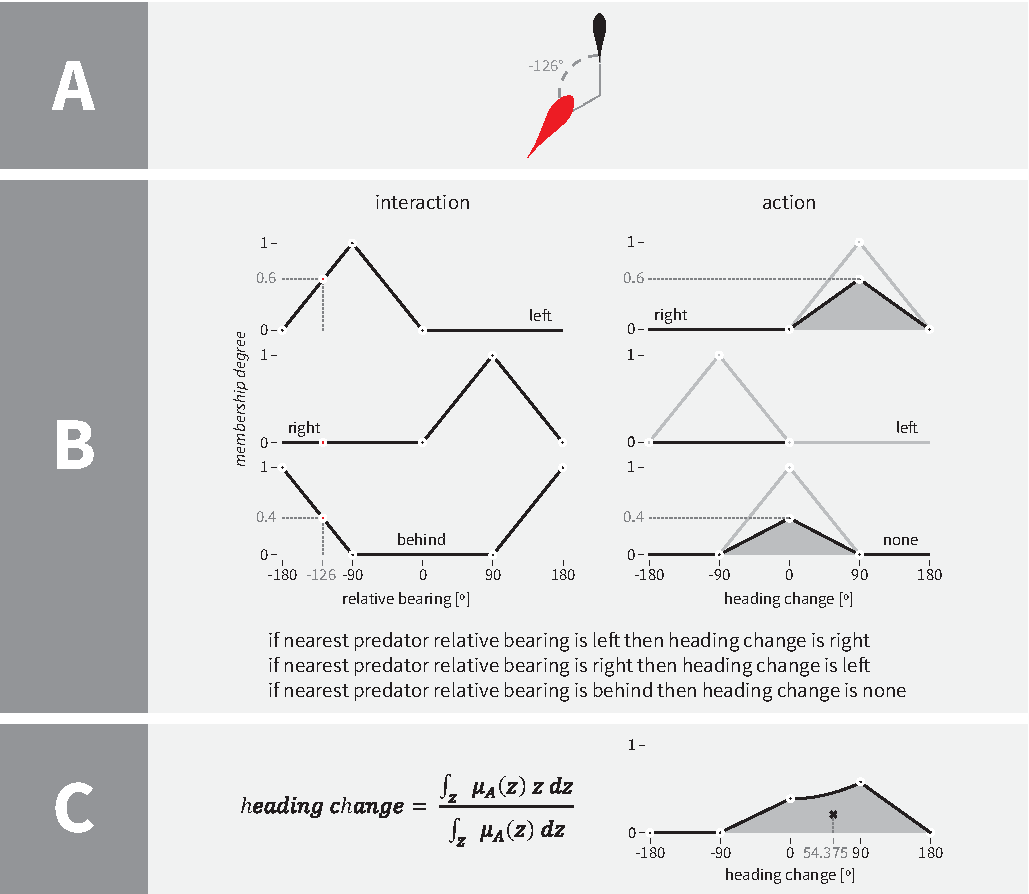
\includegraphics[width=.5\textwidth]{ecomod/fig1}
	\caption{An example of a starting configuration, where the black triangle represents the predator; its bearing is north. The shaded area is the area in which the prey group is generated. Grey dots are the prey, and the grey arrow is their average bearing.}
	\label{fig:setup}
\end{figure}

When the predator selected a target it started hunting it. Which target was selected depended on the predator's tactic -- see sections \ref{sec:mix} (\nameref{sec:mix}) and \ref{sec:dispersing} (\nameref{sec:dispersing}). The predator kept hunting the same target until the target was caught, the predator got confused, the target escaped from the predator's hunting zone radius, or the simulation time (600 steps) ran out. When the predator came close to the target, \ie within a distance that was less than the catch distance it made an attempt to catch the prey. The probability that this attempt was successful was inversely proportional to the number of individuals within the predator's confusability zone \cite{olson2013critical,olson2013predator}:
%
\begin{equation}
P_\textnormal{success}=\frac{1}{|\set{N}_\textnormal{co}|},\quad \set{N}_\textnormal{co}=\{j \in \set{A}|\ j \neq p,\ \|\vec{d}_j\| \leq r_\textnormal{co} \},
\label{eq:confusability}
\end{equation}
%
where \set{A} is the set consisting of the predator agent and prey agents, $j$ is a prey agent, $\vec{d}_j=\vec{p}_j-\vec{p}$ is the offset vector pointing from the current position of the observed agent (the predator) to the current position of agent $j$, and $r_\textnormal{co}$ is the predator's confusability zone radius.

In order to take into account the effort required to eat the prey, the predator did not look for a new target prey immediately after it had successfully caught one. A certain amount of simulation time steps, \emph{handling time} (see \tablename~\ref{tab:parameters}), had to pass before the predator selected a new target. If the predator failed to catch the targeted prey due to confusion a certain amount of simulation time steps, \emph{refocus time} (see \tablename~\ref{tab:parameters}) had to pass as well. If, however, the currently targeted prey would escape from the predator's field of view, the predator would immediately select a new target. Note that due to the choice of the model parameters, more specifically the predator and prey maximum speeds, in our model this does not happen.

In nature there are many types of prey behaving in many different ways and presumably if predators use sophisticated target selection and pursuit/hunting tactics, the prey might use sophisticated escape manoeuvres to outsmart the predator. Indeed a number of studies \cite{kunz2006prey,nishimura2002predator,olson2013predator,zheng2005behavior} suggest that confusion might play an important role in the evolution of grouping behaviour. For these reasons we ran three sets of evolutions of the two composite tactics, a) with parameters set to their default values as listed in \tablename~\ref{tab:parameters}, b) with the prey escape zone set to \BL{50}, the weight of the escape drive set to \SI{12}{\per\second\squared} and the rest of the parameters set to default, and c) with $P_\textnormal{success}$, \eq~\eqref{eq:confusability}, set to be always equal to 1 and the rest set to default. The first case, named \emph{default prey}, represents the typical scenario of a solitary predator attacking a group of prey. The second case, named \emph{prey with delayed response}, represents a group of prey that allows the solitary predator to get close and then performs a rapid escape manoeuvre. The third case, named \emph{non-confusing prey}, investigates if confusability might play a role in the evolution of target selection and pursuit/hunting tactics as well.

%-----
\subsection{Mixture of simple tactics}
\label{sec:mix}

In the first part of our research, the predator that used a mixture of simple tactics was based on similar tactics as predators presented in previous research \cite{demsar2014simulated,nishimura2002predator}: attack nearest prey, attack the most peripheral prey, and attack the most central prey. The nearest prey was simply the one that was the closest to the predator. To determine which prey was most peripheral or central we used the measure of peripherality. In previous research \cite{hemelrijk2000towards,hemelrijk2005individual,hildenbrandt2010selforganized} this measure was called centrality, but since a lower degree of centrality means that the individual is more central and less peripheral, the term peripherality is more appropriate. Peripherality of prey agent $i$ is calculated as the length of $\vec{P}_i$, \ie the average vector of direction towards the group of potentially influencing neighbours:
%
\begin{equation}
\vec{P}_i=\frac{1}{|\set{G}|} \sum_{j \in \set{G}} \uvec{d}_j,\quad \set{G}=\{j \in \set{A}|\ j \neq i,\ j \neq p,\ \|\vec{d}_j\| \leq r_\textnormal{c}\},
\label{eq:peripherality}
\end{equation}
%
where $i$ is the observed prey agent, $j$ is an agent, $p$ is the predator agent, $\uvec{d}_j=\vec{d}_j/\|\vec{d}_j\|$ the unit vector pointing from the current position of the observed agent (prey agent $i$) to the current position of agent $j$, $r_\textnormal{c}$ the prey's cohesion zone radius and $\set{G}$ the set of potentially influencing neighbours of the observed prey agent. If a prey agent was isolated (\ie the set of potentially influencing neighbours was empty) its peripherality was set to $+\infty$, meaning that the predator that targeted peripheral targets preferred to attack isolated targets \cite{ioannou2012predatory,demsar2014simulated}.

The prey that is the nearest is simply the one whose distance from the predator is the smallest: 
%
\begin{equation}
t_\textnormal{n}=t:\ \|\vec{d}_t\|=\min_{j \in \set{T}}\|\vec{d}_j\|,\ \set{T}=\{j \in \set{A}|\ j \neq p,\ \|\vec{d}_j\| \leq r_\textnormal{h}\}.
\end{equation}

The prey that is the most central is the one with the lowest measure of peripherality:
%
\begin{equation}
t_\textnormal{m}=t:\ \|\vec{P}_t\|=\min_{j \in \set{T}}\|\vec{P}_j\|,\ \set{T}=\{j \in \set{A}|\ j \neq p,\ \|\vec{d}_j\| \leq r_\textnormal{h}\}.
\end{equation}

By definition the prey that is the most peripheral is the one with the highest measure of peripherality. However, as the measure of peripherality is defined via the prey's cohesion zone radius (\ie the set of potentially influencing neighbours) and does not consider the predator's angle of approach an additional constraint was taken into account. Only prey whose peripherality vector was pointing in the same direction (\ang{\pm90}) as the unit vector pointing from the current position of the predator to the current position of the prey agent were regarded as possible targets:
%
\begin{equation}
t_\textnormal{p}=t:\ \|\vec{P}_t\|=\max_{j \in \set{T}}\|\vec{P}_j\|,\ \set{T}=\{j \in \set{A}|\ j \neq p,\ \|\vec{d}_j\| \leq r_\textnormal{h},\ \uvec{d}_j\cdot\uvec{P}_j>0\}.
\end{equation}

With this constraint we prevented the predator agent from targeting prey that were on the opposite side of the group (as viewed from the predator's point of view), because in nature they would probably not be visible to the predator.

\begin{table}
	\caption{Parameters that evolve during the evolution of a simple predator.}
	\label{tab:mix}
	\begin{tabular}{llll}
		\toprule
		Parameter & Description & Interval & Initial value \\
		\midrule
		$p_\textnormal{n}$ & Target the nearest prey probability & $[0, 1]$ & Random \\
		$p_\textnormal{m}$ & Target the most central prey probability & $[0, 1]$ & Random \\
		$p_\textnormal{p}$ & Target the most peripheral probability & $[0, 1]$ & Random \\
		\bottomrule
	\end{tabular}
\end{table}

The chromosome of the predator, which was used to construct a generation of predators, consisted of probabilities that determined the likelihood that the predator will use a particular tactic (\ie the probabilities represent genes in the chromosome). Every predator had three probabilities -- one for each of the three tactics, see \tablename~\ref{tab:mix}. For the initial generation of predators the probabilities were assigned normalized uniformly distributed random values between 0 and 1 (see \tablename~\ref{tab:mix}) so that the sum of all probabilities was equal to 1:
%
\begin{equation}
p_\textnormal{n}=\frac{\xi_\textnormal{n}}{\xi_\textnormal{n}+\xi_\textnormal{p}+\xi_\textnormal{m}},\quad p_\textnormal{m}=\frac{\xi_\textnormal{m}}{\xi_\textnormal{n}+\xi_\textnormal{p}+\xi_\textnormal{m}},\quad p_\textnormal{p}=\frac{\xi_\textnormal{p}}{\xi_\textnormal{n}+\xi_\textnormal{p}+\xi_\textnormal{m}},
\end{equation}
%
where $\xi_\textnormal{n}$, $\xi_\textnormal{m}$, $\xi_\textnormal{p}$ are uniformly distributed random values between 0 and 1, and $p_\textnormal{n}$, $p_\textnormal{m}$, $p_\textnormal{p}$ are the probabilities that the predator will attack the nearest, the most peripheral, and the most central target respectively. As already stated, at the start of an evaluation phase, the predators had no target. In the initial step of the evaluation phase the predator selected a target as:
%
\begin{equation}
t=\begin{cases}
t_\textnormal{n} & \textnormal{iff}\  \xi \in (0,p_\textnormal{n}]\\
t_\textnormal{m} & \textnormal{iff}\  \xi \in (p_\textnormal{n},p_\textnormal{n}+p_\textnormal{m}]\\
t_\textnormal{p} & \textnormal{iff}\  \xi \in (p_\textnormal{n}+p_\textnormal{m},1],
\end{cases}
\label{eq:target}
\end{equation}
%
where $\xi$ is a uniformly distributed random value in the interval $(0, 1]$, $t_\textnormal{n}$, $t_\textnormal{m}$, $t_\textnormal{p}$ are the nearest, the most central, and the most peripheral prey respectively. The target selection process, \eq~\eqref{eq:target}, was repeated every time a) the predator's attempt to catch the targeted prey was unsuccessful and the refocus time passed, or b) the predator caught the targeted prey and the handling time passed. That means that the predator could use different simple tactics on successive attacks during one simulation run (600 time steps).

In the evolution phase the chromosome of a new predator (offspring) was generated by using the coin-flip crossover, a type of crossover operator that chooses a gene from one of the parents at random (uniform distribution). The coin-flip crossover was repeated for all genes. Occasionally, being governed by the mutation rate (2\% per parameter), the genes mutated. The mutation of a specific gene, \ie probability of a specific tactic, was simulated as either an increase or a decrease (chosen at random) of the likelihood that the predator will use that particular tactic. The amount of increase/decrease was governed by the mutation factor (20\%). Because the cross-over and mutation could lead to the sum of probabilities not being equal to 1, the last step in the creation of a new chromosome was renormalization, \ie division of individual probabilities by their sum.

%-----
\subsection{The dispersing tactic}
\label{sec:dispersing}

In the second part of our study the predator's tactic was as follows. Initially (\figurename~\ref{fig:dispersing}) the predator chased the centre of the nearby group. The nearest prey (with respect to the predator) and all prey within this prey's set of potentially influencing neighbours, $\set{G}$ in \eq~\eqref{eq:peripherality}, were interpreted as the nearby group. The prey within this group that had the lowest measure of peripherality, \eq~\eqref{eq:peripherality}, \ie was the most central, was interpreted as the group's centre. The nearby group and its centre were determined once per attack and remained unchanged for the duration of the attack. Once the distance of the nearby group's centre was less than the \emph{lock-on distance} the predator locked on the most peripheral prey within its \emph{lock-on radius} (\tablename~\ref{tab:dispersing}). The locked-on individual was then hunted until captured, or the attempt failed due to confusion.

\begin{table}
	\caption{Parameters that evolve during the evolution of the dispersing predator.}
	\label{tab:dispersing}
	\begin{tabular}{llll}
		\toprule
		Parameter & Description & Interval (\si{\bodylength}) & Initial value\\
		\midrule
		$d_\textnormal{l}$ & Lock-on distance & $[0, 400]$ & Random\\
		$r_\textnormal{l}$ & Lock-on radius & $[0, 400]$ & Random\\
		\bottomrule
	\end{tabular}
\end{table}

\begin{figure}
	\vskip.4in % add top and bottom whitespace so that the caption does not overflow the figure box 
	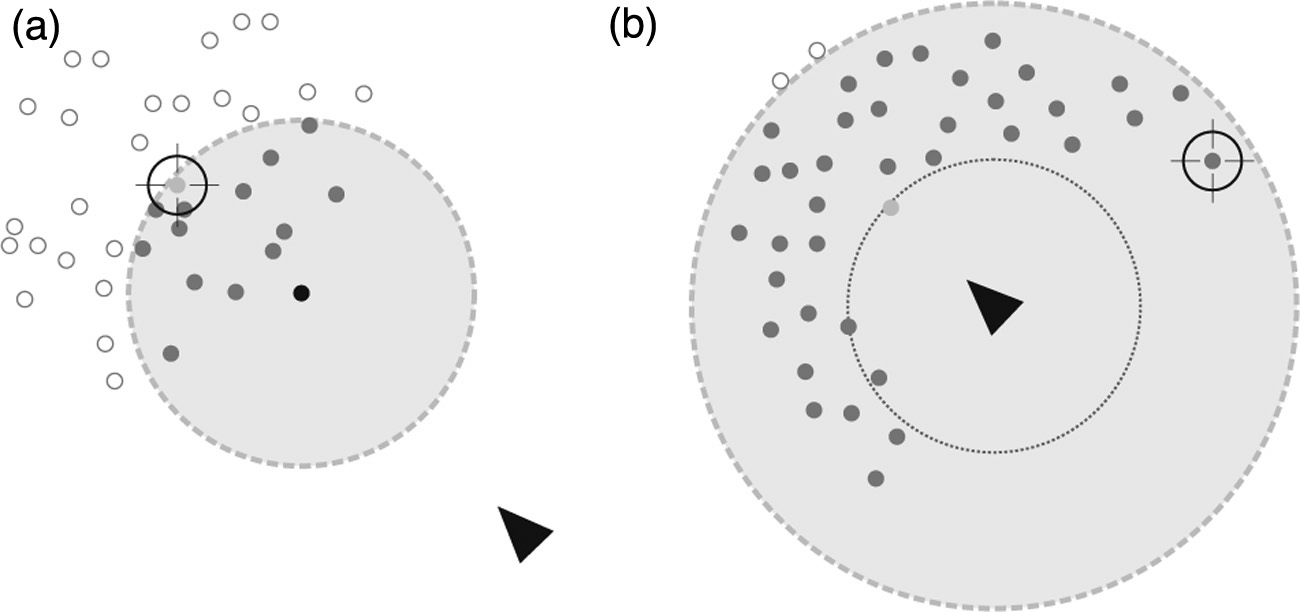
\includegraphics[width=.95\figurewidth]{ecomod/fig2}
	\vskip.4in
	\caption{The dispersing tactic; a predator (black triangle) that uses this tactic initially (a) chases the most central prey (light grey dot) in the nearby group of prey, grey dots, (\ie prey that are within the cohesion zone radius, shaded area, of the nearest prey, black dot). When the predator comes close enough (b), \ie within lock-on distance, dotted circle, it selects as its target prey the most peripheral prey within its lock-on zone radius, shaded area.}
	\label{fig:dispersing}
\end{figure}

During the evolution phase the predators that caught more prey in the evaluation phase had a higher chance of being selected as parents. The offspring predator inherited the value of the lock-on distance from the first parent and the value of the lock-on radius from the second parent. Once in a while the parameters would mutate; the probability of mutation was governed by the mutation rate (2\% per parameter). The mutation was in the form of either an increase or decrease (chosen at random) and the amount was governed by the mutation factor (20\%). The parameters that evolved during our experiments and their initial values can be seen in Table \ref{tab:dispersing}.

%-----
\section{Results and Discussion}

\paragraph{Mixture of simple tactics} In the first part of our research we investigated which of the simple tactics an evolved solitary predator will resort to use the most. This was measured by observing the probabilities that determined the likelihood that a particular tactic would be employed. \figurename~\ref{fig:mix:evo} shows the averages and bootstrapped 95\% confidence interval of the 20 runs for the cases of default prey, prey with delayed response and non-confusing prey. 

\begin{figure}
	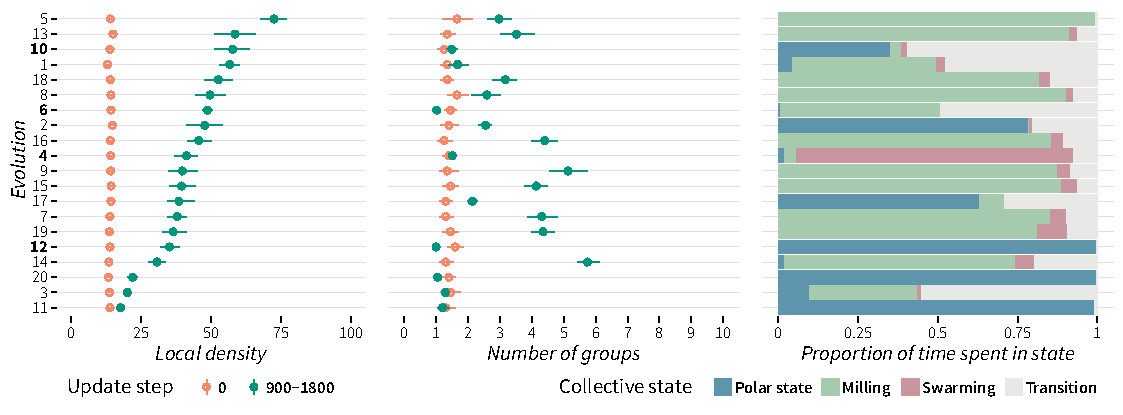
\includegraphics[width=\figurewidth]{ecomod/fig3}
	\infigurecaption{Averages and the bootstrapped 95\% confidence intervals based on 20 replicates of our experiments in three different settings -- predators facing a group of prey with default parameters as in Table \ref{tab:parameters} (default prey), predators facing a group of prey with a delayed response, and predators with confusability radius set to 0 (non-confusing prey).}
	\caption{Evolution of the probabilities that determine the likelihood that the predator will use a particular simple tactic when choosing its next target.}
	\label{fig:mix:evo}
\end{figure}

As it can be seen, in the case of default prey, an evolved predator (predator of the last, 500th, generation) attacked almost exclusively the most peripheral prey, 96\% \ci{95.6}{96.9}, meaning that during the course of the evolution predators that attacked the most peripheral targets were more successful than those whose ratio of attacking the nearest or most central prey was higher. For this reason the probability of using these two tactics was very low, 2\% \ci{1.9}{3} and \num{1.3}\% \ci{1}{1.7}, respectively.

In the case of prey with delayed response the evolved predator again mainly attacked the most peripheral prey, 84\% \ci{75}{88.5}. The decrease in probability was mostly due to the increase of the probability of attacking the nearest prey, 12\% \ci{7.3}{20.8}, while the probability of attacking the most central prey still remained very low 4\% \ci{3.6}{4.8}. The adaptation seems quite reasonable as due to the prey's delayed response there is also a higher chance of success when attacking the nearest prey as it might not be able to escape due to overcrowding.

In the case of non-confusing prey, however, the evolved predator adapted to attacking the most central, 55\% \ci{37.5}{71.3}, and nearest prey, 40\% \ci{23.4}{56}. In this case the probability of attacking the most peripheral prey was very low 5\% \ci{4.3}{6}. This result again seems reasonable as attacking peripheral prey builds on the reduction of the chance of the predator getting confused due to the abundance of prey in the vicinity of the chosen target.

\paragraph{Dispersing tactic} In the second part of our research we investigated how an evol\-ving solitary predator that uses the dispersing tactic will adapt the distance at which it will stop chasing the centre of the nearest group and select its actual target prey individual, as well as the radius within which it will search for it. In \figurename~\ref{fig:dispersing:evo}, which shows the means and bootstrapped 95\% confidence interval of the 20 runs for the cases of default prey, prey with delayed response and non-confusing prey, it can be seen that in the case of default prey the evolved predator (predator of the last, 500th, generation) stopped chasing the centre of the nearest group when \BL{19} \ci{18.5}{20.2} from it. Then it locked-on the most peripheral prey in a radius of \BL{129} \ci{112.4}{147}.

\begin{figure}
	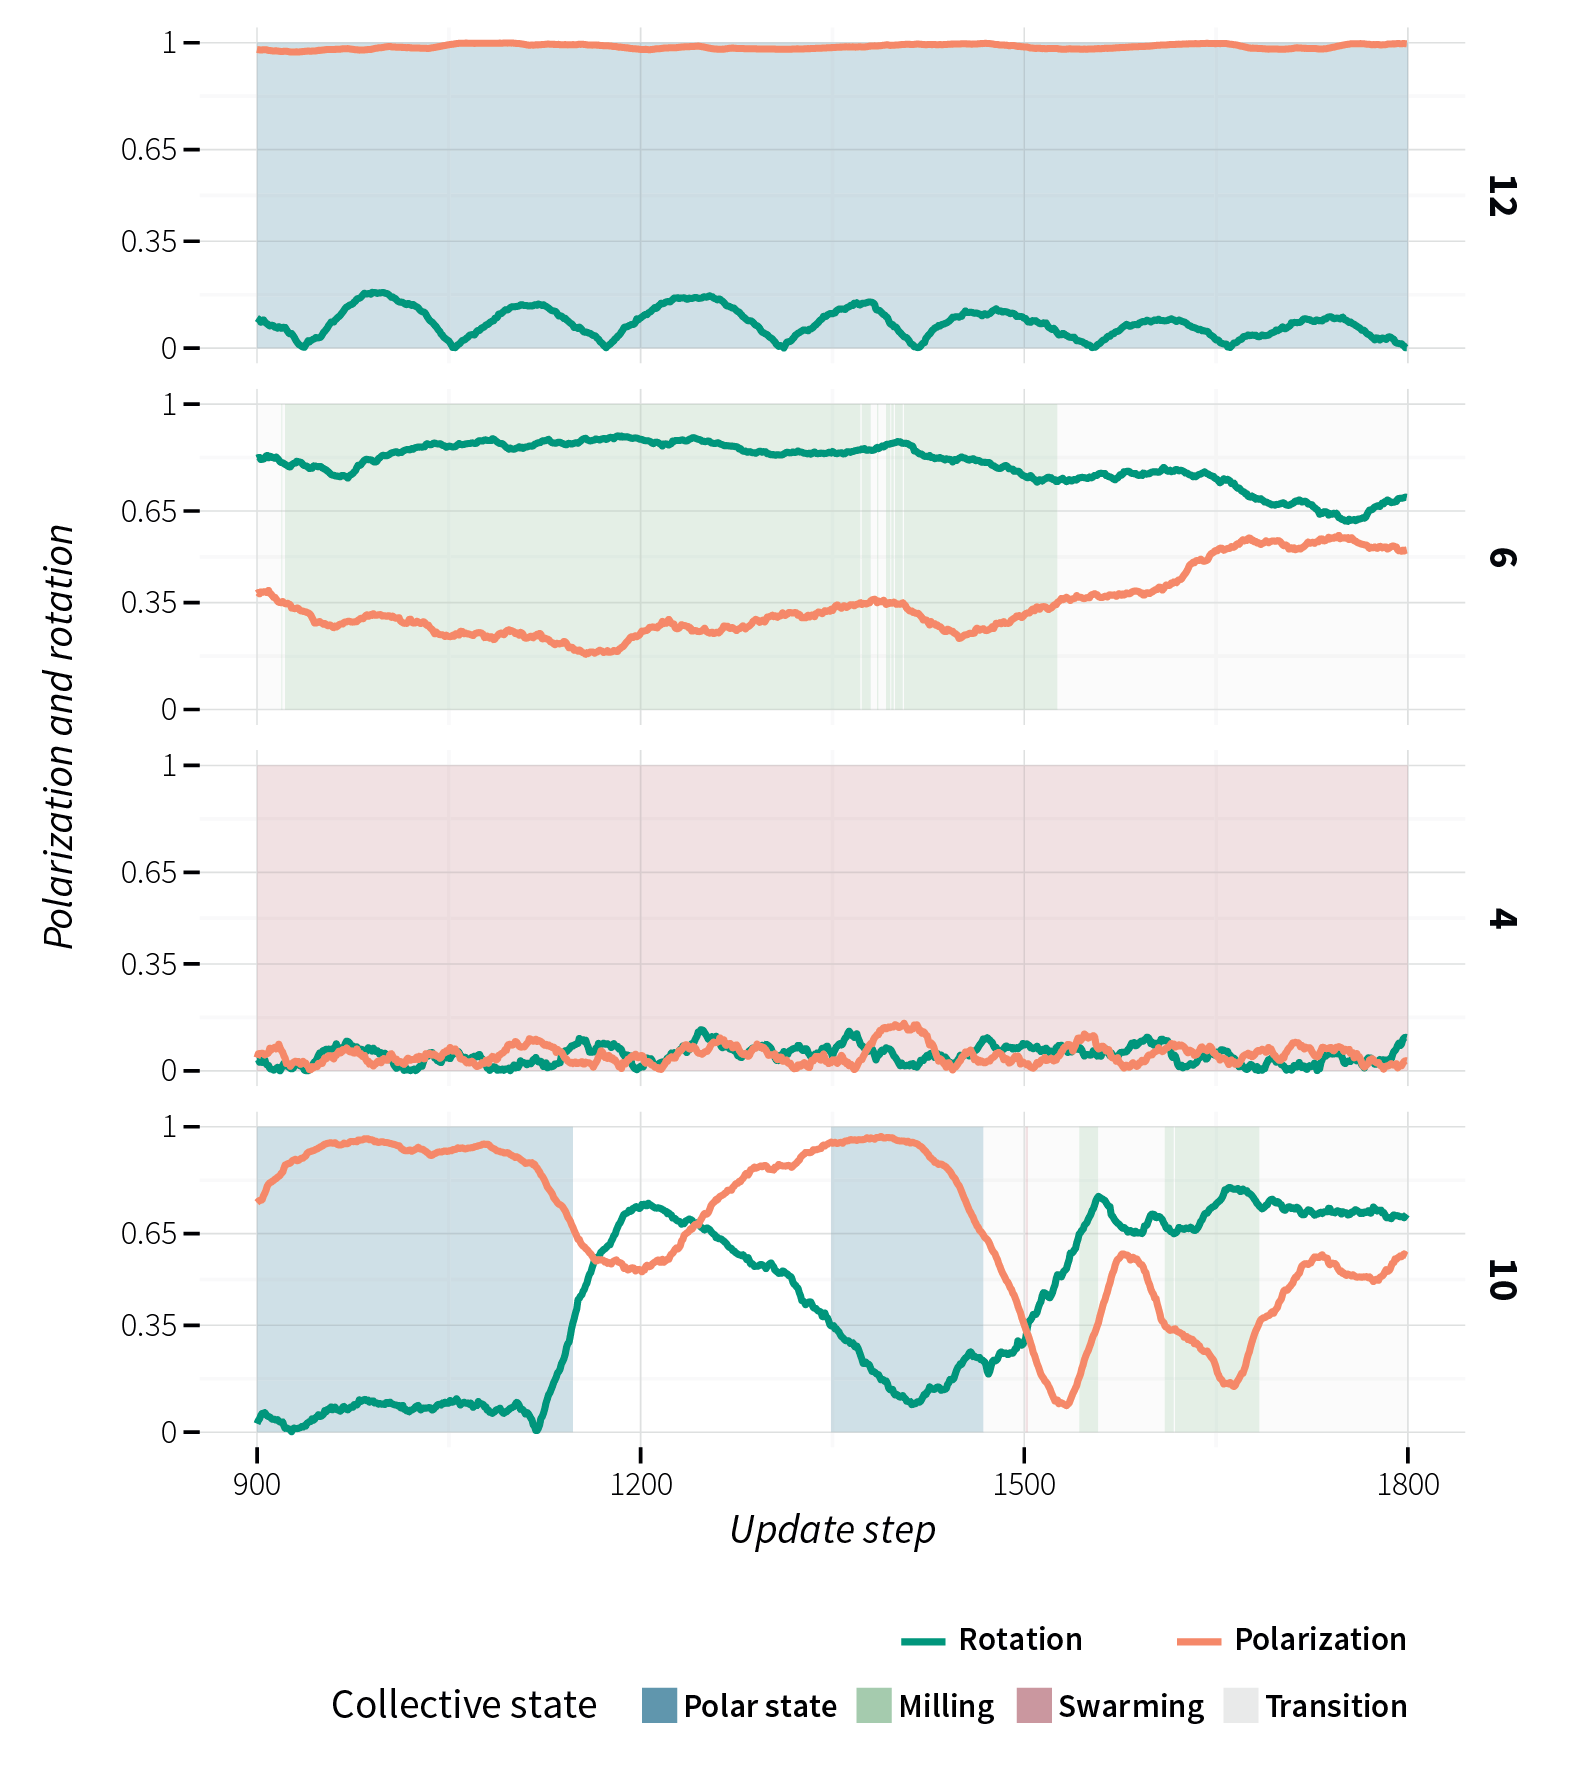
\includegraphics[width=\figurewidth]{ecomod/fig4}
	\infigurecaption{Averages and the bootstrapped 95\% confidence intervals based on 20 replicates of our experiments in three different settings -- predators facing a group of prey with default parameters as in Table \ref{tab:parameters} (default prey), predators facing a group of prey with a delayed response, and predators with confusability radius set to 0 (non-confusing prey).}
	\caption{Evolution of the lock-on distance and lock-on radius in the case of the dispersing predator.}
	\label{fig:dispersing:evo}
\end{figure}

In the case of prey with delayed response the chasing stopped when \BL{12.8} \ci{11}{14.4} away from the centre of the nearest group and the final target was searched within \BL{103} \ci{77.8}{129.4}. Interestingly, in the case of prey with delayed response, the predator adapted to dive significantly deeper \BLpss{2.5} (\ttest{-6.7227}{29.757}{9.832e-8}) but there was no significant difference between the radii within which the final targets were chosen (\ttest{-1.6589}{33.869}{0.1064}).

In both cases the predator locked on its target when it came quite close to the centre of the nearest group. As possible values for the lock-on distance ranged from 0 to \BL{400} we can assume that dispersing a school, flock or herd greatly reduces its defensive benefits. When the evolved predator locked on its target, it locked on the most peripheral prey in a radius that is lower than the midpoint of possible values (0 to \BL{400}), therefore we can assume that in both cases the dispersing predator preferred isolated but somewhat nearby prey. This suggests that the best potential targets might be prey that are close to the periphery of a school, flock, or herd while at the same time somewhat close to the predator.

In the case of non-confusing prey, however, the chasing stopped when \BL{153} \ci{148.5}{156.3} from the centre of the nearest group, and the final target was searched within \BL{151} \ci{147.6}{154}. Surprisingly there was no significant difference between the two parameters (\ttest{0.561}{36.83}{0.5782}). What is even more interesting is that the values are close to the midpoint of possible values (0 to \BL{400}), and since there is no significant difference between the two values, the end result is a behaviour very similar to attacking the nearest prey. Note that the dispersing predator initially chases the centre of the nearest group and when close enough locks-on the most peripheral target within the lock-on radius. Since the lock-on radius and lock-on distance are very similar, the end result is that the nearest prey and most peripheral prey within the searched radius often coincide.

\paragraph{Comparison between tactics via direct competition} In the third part of our research we used direct competition in order to assess the quality of the evolved tactics from the predator's point of view. Each individual predator that emerged from the 20 replicates of an experiment (mixture of simple tactics, and dispersing tactic) was released to independently attack the same \num{1000} distinct groups of prey, each for 600 time steps and the number of caught prey recorded. This was repeated 3 times, a) with 1000 distinct groups of default prey, b) with 1000 distinct groups of prey with delayed response, and c) with 1000 distinct groups of non-confusing prey. As a control group we also observed the number of caught prey for predators that a) attacked random prey, b) always attacked the most peripheral prey, c) always attacked the nearest prey, and d) always attacked the most central prey. In total \num{600000} simulations were performed and \figurename~\ref{fig:mvsd} presents the distributions, boxplots and averages of the distributions of the number of caught prey per tactic per specific setting.

\begin{figure}
	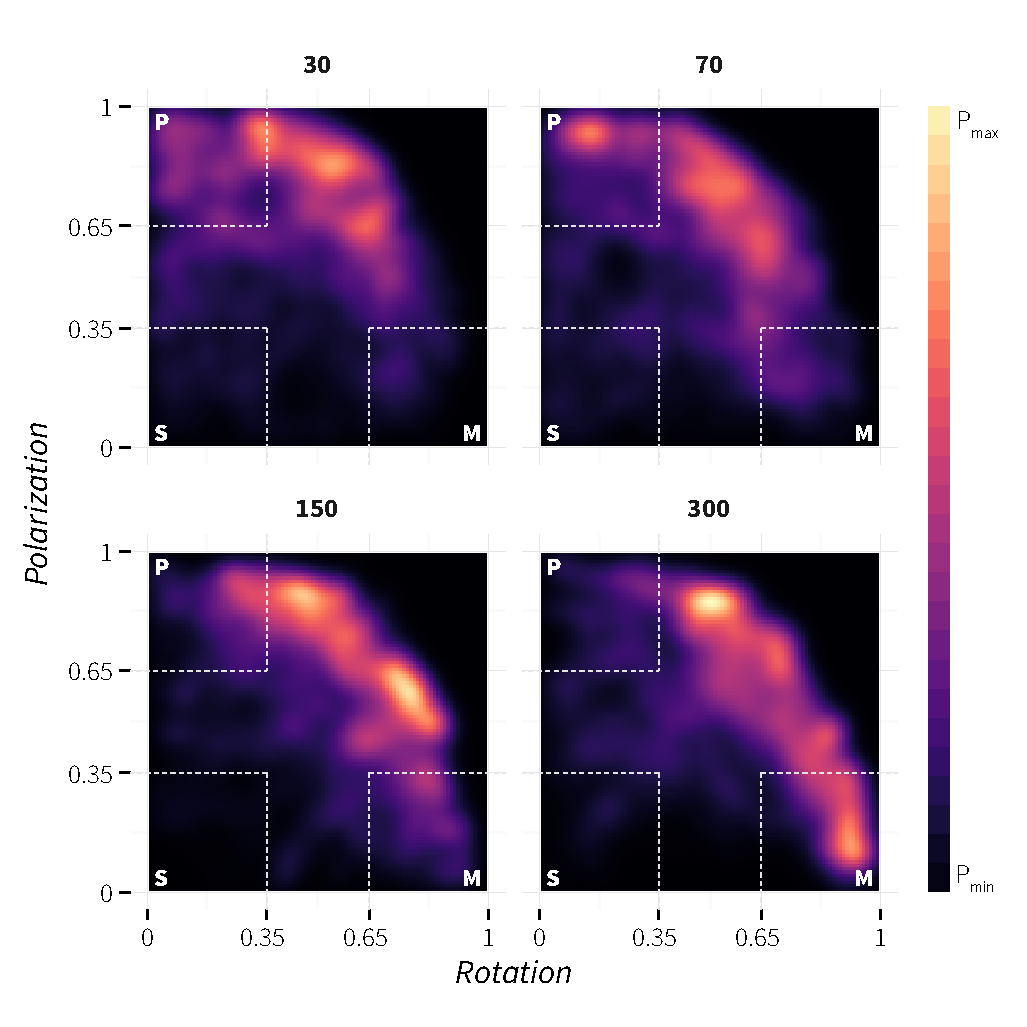
\includegraphics[width=\figurewidth]{ecomod/fig5}
	\caption{Results of a direct competition between the individual predators that emerged from the 20 replicates of each of our experiments and a control group consisting of predators that attack exclusively the most peripheral prey, exclusively the nearest prey, exclusively the most central prey, or a random individual. Presented are the distributions, boxplots and averages of the distributions of the number of caught prey per tactic per specific setting.}
	\label{fig:mvsd}
\end{figure}

The number of caught prey in general ranged from 0 to 9 in a single 600 time steps long run. In the cases of default prey and prey with delayed response the number of caught prey ranged only from 0 to 6 and 0 to 7, respectively, and the averages were \num{1.522} \ci{1.517}{1.527} and \num{1.327} \ci{1.322}{1.332}, respectively. In the case of non-confusing prey the average was substantially higher, \ie \num{5.357} \ci{5.35}{5.363}. The lowest average number of caught prey was thus in the case of prey with delayed response and the highest in the case of non-confusing prey. This suggests that a delayed response might be a successful advanced defence tactic against predation, a response to predator attacks that is not uncommon in nature \cite{partridge1982structure}.

In the case of default prey the most successful predator was the predator that used the dispersing tactic with the tactic's parameters adapted to default prey, it caught on average \num{2.773} \ci{2.757}{2.787} prey. The next best was the dispersing predator with the tactic's parameters adapted to prey with delayed response, which caught on average \num{2.707} \ci{2.69}{2.725} prey. Third best, with a substantial gap of approximately 34\%, were the predators that attacked exclusively the most peripheral prey with an average of \num{1.704} \ci{1.69}{1.717} and the predator that used the mixture of simple tactics with parameters adapted to default prey, whose average was \num{1.684} \ci{1.67}{1.698}. The difference between these two tactics was statistically not significant (\ttest{2.0661}{39991.2}{0.03882}), which is not surprising as the predator that uses the mixture of simple tactics adapted to default prey in roughly 96\% of cases attacks the most peripheral prey. Composite tactics (mixture of simple tactics, and dispersing tactic) adapted to prey with delayed response registered lower averages than those adapted to default prey; in both cases the difference was less than 5\%. Not surprisingly the composite tactics adapted to non-confusing prey fared the worst from the three possible adaptations, but surprisingly the dispersing tactic adapted to non-confusing prey with an average of \num{1.412} \ci{1.396}{0.1428} came sixth and still had a higher success rate than attacking exclusively the nearest prey \CI[1.218]{1.203}{1.233}. Interestingly as well, attacking exclusively the most central prey came in last with an average of \num{0.515} \ci{0.505}{0.525}, worse even than attacking random prey whose average was \num{0.784} \ci{0.772}{0.794}.

In the case of prey with delayed response the average number of caught prey lowered, but the dispersing tactic yet again turned to be the best tactic. This time the best tactic was the dispersing tactic with parameters adapted to prey with delayed response, with an average of \num{2.429} \ci{2.412}{2.447}, followed by the dispersing tactic adapted to default prey, with an average of \num{2.113} \ci{2.093}{2.133}. Again, with a substantial gap of roughly 37\%, the third best tactic were attacking exclusively peripheral prey and, surprisingly, the mixture of simple tactics adapted to default prey, with averages of \num{1.337} \ci{1.324}{1.351} and \num{1.327} \ci{1.314}{1.341}, respectively. As in the case of default prey there was no significant difference between the two tactics (\ttest{-1.0239}{39997.72}{0.3059}). Interestingly in the case of the mixture of simple tactics the adaptation to the specific setting did not help, the mixture of simple tactics adapted to prey with delayed response with an average of \num{1.293} \ci{1.279}{1.306} actually performed worse than the one adapted to default prey (\ttest{-3.3619}{39997.83}{0.0003874}). The results seem to suggest that although from the prey's point of view delaying the response might be a successful advanced defence tactic against predation, certain composite predation tactics, like the dispersing tactic, could potentially adapt and at least partially diminish its effectiveness. Surprisingly the dispersing tactic adapted to non-confusing prey, with an average of \num{1.248} \ci{1.234}{1.263}, again came in sixth, but this time reduced the gap to the mixture of simple tactics adapted to prey with delayed response from 12\% to merely 4\%. As in the case of default prey, worse even than attacking random prey, whose average was \num{0.74} \ci{0.729}{0.751}, was attacking exclusively the most central prey, the worst tactic of all, but this time with a higher average of \num{0.695} \ci{0.686}{0.706}. The substantial, 35\%, increase in success rate might be attributed to the fact that delaying the response to a predator attack also increases the chance for prey to be unable to escape due to overcrowding.

In the case of non-confusing prey the picture was completely different. The average number of caught prey was obviously substantially higher as once the predator selected its target it was impossible for the predator to fail catching the targeted prey. Hence the difference in tactics came from the amount of time that was lost during pursuit and the most successful tactics were the ones that successfully mitigated between the abundance of possible targets and the distance that had to be travelled for the next kill. This time the best tactic was to attack the nearest prey, with an average of \num{6.412} \ci{6.397}{6.426}, closely followed by the mixture of simple tactics adapted to non-confusing prey, with an average of \num{6.307} \ci{6.295}{6.318}, and attack the most central prey \num{6.258} \ci{6.25}{6.266}. The dispersing tactic adapted to non-confusing prey came in fourth with an average of \num{6.004} \ci{5.989}{6.019}. Not surprisingly, as in the case of non-confusing prey the adaptations of the two composite tactics were closely related to the two best tactics (attack the nearest prey and attack the most central prey). Indeed, recall that the mixture of simple tactics adapted to attacking the most central prey in 55\% of cases and attacking the nearest prey in 40\% of cases. Similarly the adaptation of the dispersing tactic was to have the lock on distance and lock on radius almost the same (\BL{153} and \BL{151}, respectively), which could be interpreted as attacking the nearest prey, even more so because the prey started escaping when the predator was \BL{100} from it. Surprisingly, the tactic where the predator attacked random prey came in fifth, with an average of \num{5.316} \ci{5.298}{5.334}. This was followed by the mixture of simple tactics adapted to prey with delayed response, with an average of \num{5.135} \ci{5.116}{5.153}, mixture of simple tactics adapted to default prey, with an average of \num{4.91} \ci{4.891}{4.927}, and attacking exclusively the most peripheral prey, with an average of \num{4.825} \ci{4.807}{4.842}. Interestingly, in contrast to the other two cases in this case there was a statistically significant difference between the mixture of simple tactics adapted to default prey and the tactic of attacking exclusively peripheral prey (\ttest{-6.4742}{39997.49}{9.644e-11}). This could be attributed to the small, but obviously important, 2\% and 1\% probability that the predator using the mixture of simple tactics adapted to default prey will attack the nearest or most central prey, respectively. What is even more interesting is that the dispersing tactics adapted to default prey and the dispersing tactic adapted to prey with delayed response fared the worst, with averages of \num{4.301} \ci{4.286}{4.318} and \num{4.1} \ci{4.081}{4.116}, respectively. The results suggest that confusion might not play an important role only in the evolution of schooling like previous studies suggest \cite{kunz2006prey,nishimura2002predator,olson2013predator,zheng2005behavior}, but also an important role in the evolution of sophisticated predator target selection, pursuit/hunting and prey evasion tactics. As Lett\etal \cite{lett2014effects} showed frequent sequential attacks are a good tactic for disturbing a prey school and intuitively it seems that the success of a specific tactic could be attributed to the frequency of sequential attacks, but we reserve the study of this particular case for future research.

%-----
\section{Conclusion}

Most of the existing research on the evolution of collective behaviour concentrates on the behaviour of prey under threat of predation. Even research that studies the co-evolution of collective behaviour and attack tactics or deals with attack tactics alone concentrates mainly on simple tactics (attack nearest prey, attack the most central prey, attack the most peripheral prey) \cite{demsar2014simulated,kunz2006prey,nishimura2002predator,olson2013critical,olson2013predator,olson2016evolution}. In this study we investigated two composite tactics a) a tactic where the predator in successive attacks based on probability chooses one of several simple attack tactics (mixture of simple tactics), and b) the dispersing tactic, where the predator intentionally defers the decision about its actual target to a later point in time. Both tactics were evolved in three settings, one default, and two special, namely a) on prey with delayed response and b) on non-confusing prey. A direct competition between the evolved predators (instances of tactic parameters adapted to specific settings) of 600\,000 simulations revealed that attacking the nearest prey or the most central prey is the best tactic when confusability is not at play, while simply attacking a random individual is not far behind (with only a 17\% lower success rate than attacking the nearest prey). The competition results suggest that confusability might play an important role in the evolution of target selection/hunting tactics and/or prey evasion tactics. The competition results show that the dispersing tactic is the best tactic when confusability is at play. Additionally, the results suggest that advanced evasion tactics, like a delayed response \cite{partridge1982structure}, are from the prey's point of view successful as they generally reduce the number of caught prey, but also that the dispersing tactic is capable of adapting to at least partially counter the effect. The adaptation is simply diving deeper into the group of prey before selecting the final target.

%-----
\chapterAcknowledgements{We sincerely thank Frank H. Heppner of the University of Rhode Island, and Maja Lebar Bajec for reading early drafts of the manuscript. We would also like to thank the anonymous reviewers whose suggestions greatly improved the quality and clarity of this manuscript. The work is part of the PhD thesis that is being prepared by J.~Demšar at the Faculty of Computer and Information Science, University of Ljubljana, Slovenia, in collaboration with the Behavioural ecology and Self-organization group, University of Groningen, The Netherlands. It was funded in part by the Slovenian Research Agency (ARRS) through the Pervasive Computing research programme (P2-0395) and in part by the Slovene Human Resources Development and Scholarship Fund through the International Research Cooperation for PhD Students in 2012 (146.~JR) funding scheme.}

\clearpage % force supplementary material section to appear on next page

%=====
\begin{subappendices}

%-----
\section{Supplementary material}

\begin{video}[!h] % force figure to appear after section heading
	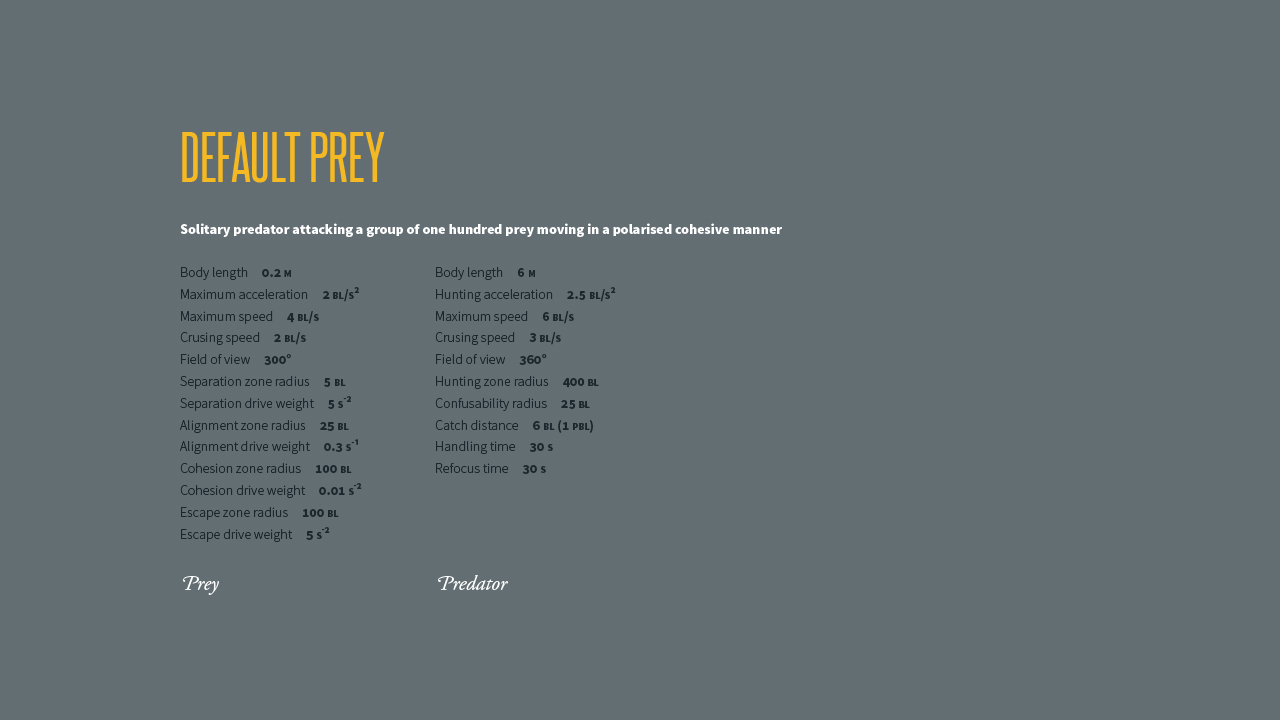
\includegraphics[width=\figurewidth]{ecomod/video_Default}
	\caption{Solitary predator attacking a group of one hundred prey moving in a polarised cohesive manner. Comparison between predator attack tactics: attacking a random prey, attacking the most central prey, attacking the nearest prey, attacking the most peripheral prey, mixture of simple tactics, dispersing tactic. Available online at \href{https://vimeo.com/119847644}{vimeo.com/119847644}.}
	\label{video:V1:ecomod}
\end{video}

\begin{video}[!hb] % force figure to appear on same page
	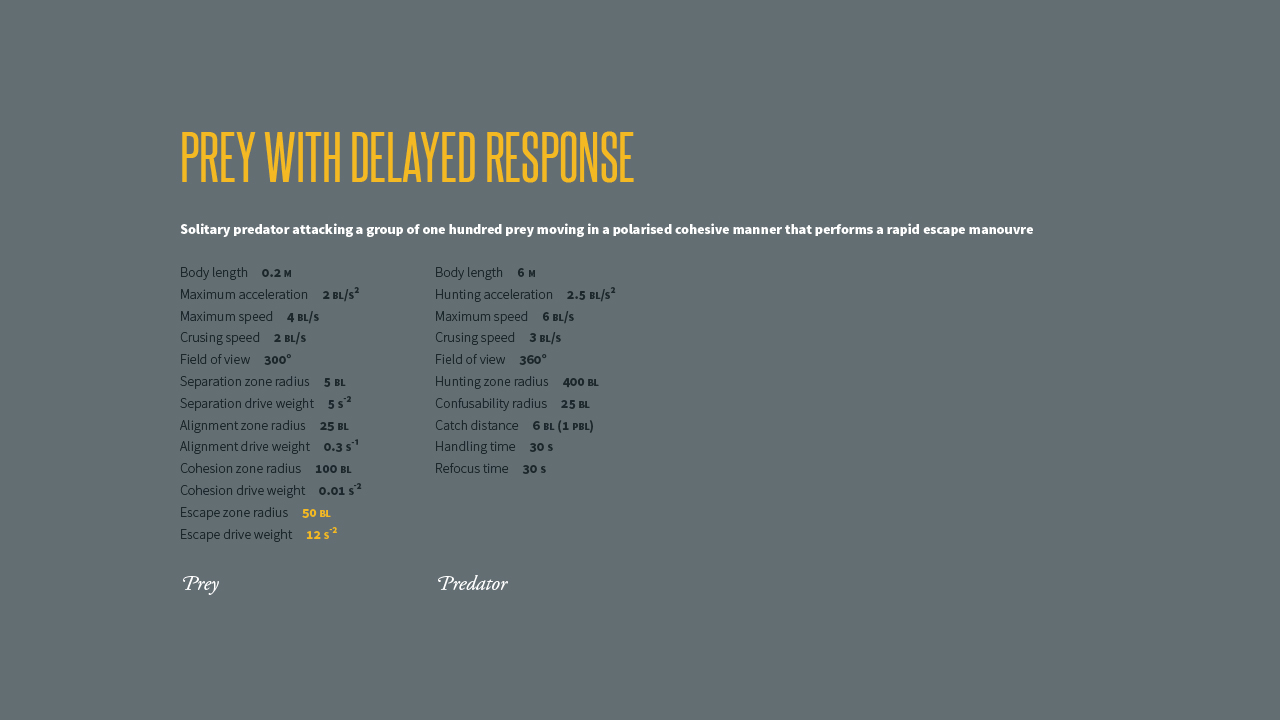
\includegraphics[width=\figurewidth]{ecomod/video_Delayed}
	\caption{Solitary predator attacking a group of one hundred prey moving in a polarised cohesive manner. Comparison between predator attack tactics for the case of prey with a delayed response: attacking a random prey, attacking the most central prey, attacking the nearest prey, attacking the most peripheral prey, mixture of simple tactics, dispersing tactic. Available online at \href{https://vimeo.com/119847316}{vimeo.com/119847316}.}
	\label{video:V2:ecomod}
\end{video}

\begin{video}[p]
	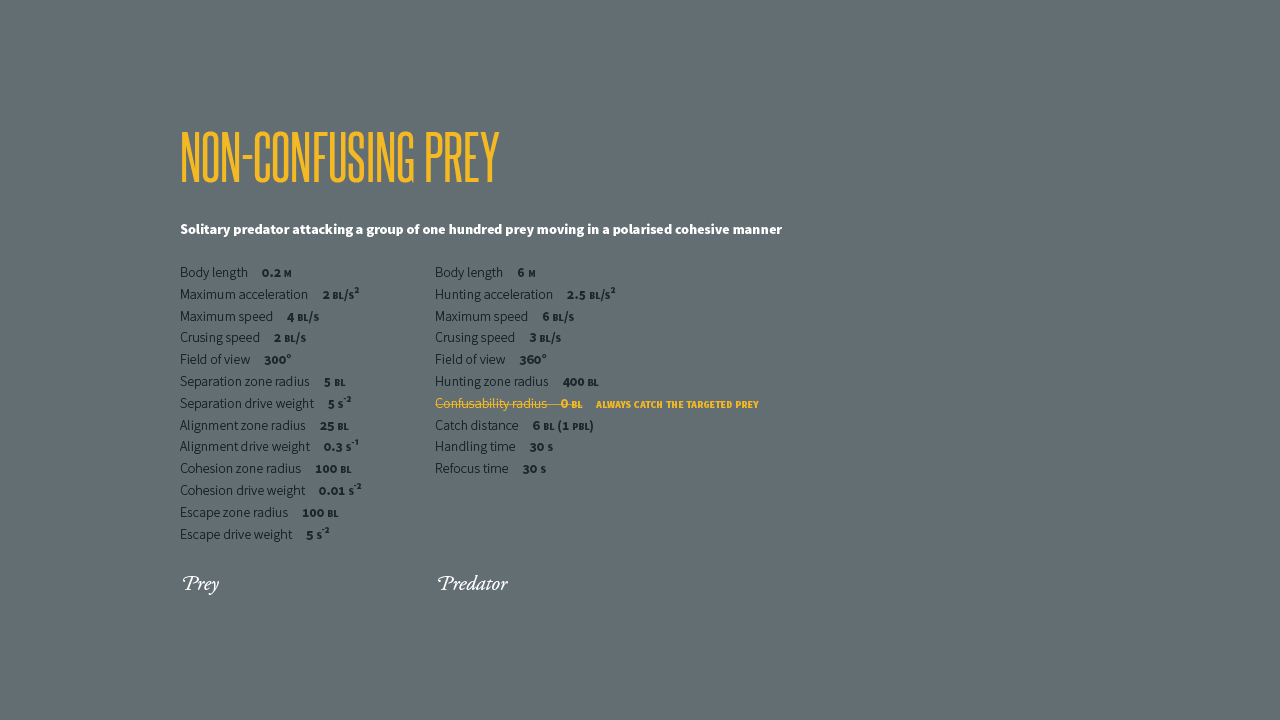
\includegraphics[width=\figurewidth]{ecomod/video_NC}
	\caption{Solitary predator attacking a group of one hundred prey moving in a polarised cohesive manner. Comparison between predator attack tactics for the case of non-confusing prey: attacking a random prey, attacking the most central prey, attacking the nearest prey, attacking the most peripheral prey, mixture of simple tactics, dispersing tactic. Available online at \href{https://vimeo.com/119846051}{vimeo.com/119846051}.}
	\label{video:V3:ecomod}
\end{video}

\end{subappendices}
